\section{Hardware}

\subsection{Grundlagen}
\label{sec:basics}

\subsubsection{Arten von VR Headsets}
\label{sec:vr-headset-types}

Bei VR Headsets werden grundsätzlich drei verschiedene Arten unterschieden:

\begin{itemize}
    \item Tethered Headsets
    \item Standalone Headsets
    \item Smartphone und Handheld Headsets
\end{itemize}

In Folge werden diese Arten kurz beschrieben, sodass die beschreibungen von der Technologien verstanden werden können.
Für eine genauere beschreibung dieses Themas wird auf~\cite{ANIWAA_TEAM_2021} verwiesen.

\emph{Tethered VR Headsets} müssen immer mit einem Computer verbunden sein, weil die VR-Applikation ausschließlich auf dem Computer läuft.
Die Brille hat dabei einerseits die Funktion die vom Computer gerenderten daten darzustellen und andererseits Positionsdaten an den Computer zurückzusenden, damit diese in der Applikationslogik verwendet werden können, um zukünftige Bilddaten zu rendern.

Bei \emph{Standalone VR Headsets} ist in der Brille ein Computer integriert, auf welchem die VR Applikation läuft.
Der Computer dient ausschließlich aus Entwicklungsplattform und die fertigen Applikationen müssen auf die Brille heruntergeladen werden.

Im Falle des \emph{Smartphone VR Headsets} läuft die Applikation auf einem Smartphone.
Um die Immersion zu erhöhen wird das Smartphone in die VR-Brille eingeschoben.
In diesem Fall dient das Telefon sowohl als Anzeigegerät als auch als Sensordatenprovider.
Die VR-Brille besteht ausschließlich aus Linsen welche die Immersion der am Handy laufenden Applikation erhöht.

\subsubsection{Tracking}

Unter Tracking versteht man das ermitteln der Position von Objekten in der realen Welt.
Folgend werden Arten das Tracking beschrieben.
Diese beinhalten:

\begin{itemize}
    \item Outside In Tracking
    \item Markerless Inside Out Tracking
    \item Marker Based Inside Out Tracking
\end{itemize}

Wie im vorigen Abschnitt wird hier nur ein Überblick über diese Arten des Trackings gegeben.
Für nähere Informationen wird auf~\cite{Dennis_Ziesecke_2019} verwiesen.

\emph{Outside In Tracking} beschreibt das Ermitteln der Positionen durch außenstehende Sensoren.
Das bedeutet, dass das zu trackende Objekt nicht weiß wo es sich im Raum befindet (Es ist passiv).
Währenddessen ermitteln außenstehende Sensoren die Position der zu trackenden Objekte und gibt diese an die VR-Applikation weiter.

Im Gegensatz dazu gibt es das \emph{Inside Out Tracking}.
Hier ermitteln Sensoren, welche sich auf den Objekten befinden die Position derselbigen.
Dabei gibt es zwei verschiedene Arten, welche bereits oben aufgelistet worden sind.

Im Fall von \emph{Markerless Inside Out Tracking} wird natürliches Licht verwendet.
Typischerweise werden hierbei Kameras verwendet.
Die dabei aufgenommenen Bilder werden mithilfe von Bildverarbeitungsmethoden analysiert und somit wird die Position der Objekte ermittelt.

Bei \emph{Marker Based Inside Out Tracking} wird im Gegensatz kein natürliches Licht verwendet.
Hierbei ist sind die zu trackenden Objekte von Lighthouses (siehe Abschnitt~\ref{sec:lighthouse}) abhängig.
Diese beleuchten den Raum mit nicht sichtbaren licht welches von Fotosensoren an den Geräten empfangen wird.


\subsection{VR Headset}
\label{sec:vr-headset}
\setauthor{Quirin Ecker}

Es sind einige VR Headsets auf dem Markt.
Nach einer Statistik aus 2017 sind die beliebtesten VR Headset Hersteller Sony, Oculus und HTC (Siehe Abb.~\ref{fig:vr_headset_manufacturer_marketshare}).
Folgend sind 3 VR Brillen beschrieben.
Hierbei wurden die auf die Spielkonsolen-basierten VR Headsets nciht berücksichtigt.

\begin{figure}
    \centering
    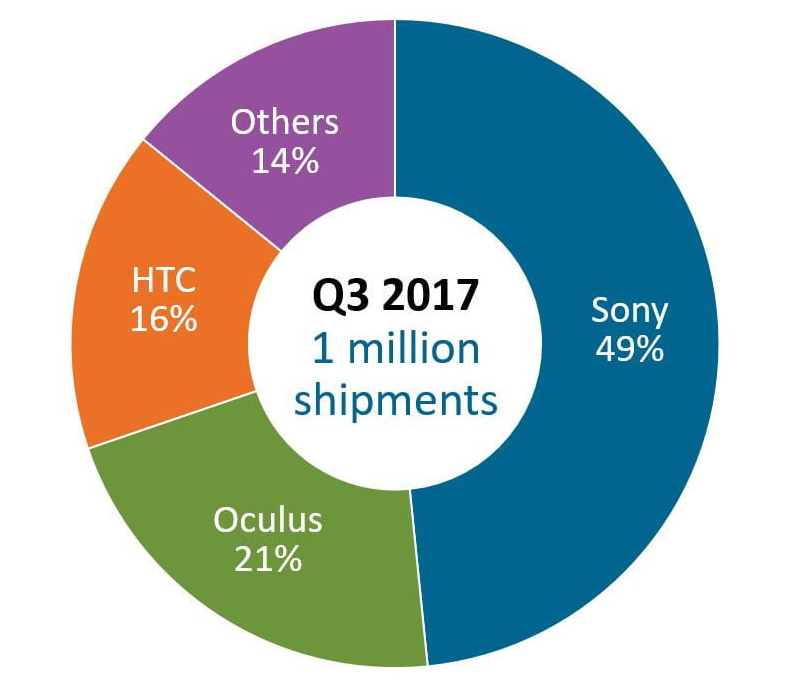
\includegraphics[scale=0.25]{pics/vr_headset_manufacturer_marketshare}
    \caption{Market-share VR Headset Hersteller~\cite{MARTINDALE_2017}}
    \label{fig:vr_headset_manufacturer_marketshare}
\end{figure}

\subsubsection{HTC Vive Pro}\label{sec:htc-vive}

Wie bereits in Abschnitt~\ref{sec:vr-headset-types} beschrieben, gibt es von diesen Headsets verschiedene Modelle.
Die HTC Vive Pro ist vom Typ ein tethered Headset mit dem Zusatz, dass auch sogenannte Light Houses gebraucht werden (siehe Abschnitt~\ref{sec:lighthouse}).
Andere Produkte, wie die im Folgendem beschriebene Oculus Quest benötigen solche nicht.

\paragraph{Vorteile}

\begin{itemize}
    \item die HTC kann mit SteamVR verwaltet werden, womit der manuelle Download von externer Software vermieden wird.
    \item lighthouse tracking
    \begin{itemize}
        \item genaueres tracking~\ref{fig:tracking_precision_statistic}
        \item nicht von dem natürlichen Licht abhängig~\cite{Dennis_Ziesecke_2019}
    \end{itemize}
\end{itemize}

\begin{figure}
    \centering
    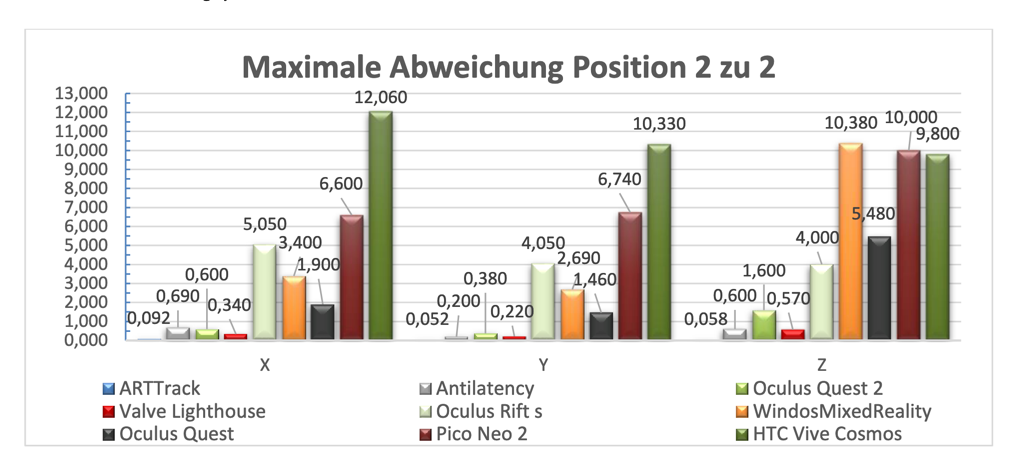
\includegraphics[scale=0.4]{pics/tracking_precision_statistic}
    \caption{Tracking Genauigkeit der VR Headsets~\cite{Macedo_2020}}
    \label{fig:tracking_precision_statistic}
\end{figure}

\paragraph{Nachteile}

\begin{itemize}
    \item längerer Aufbau wie die Folgend beschriebene Oculus Quest 2
    \item hoher Preis~\ref{fig:vr_headset_prices}
    \item es wird ein Computer benötigt
\end{itemize}

\begin{figure}
    \centering
    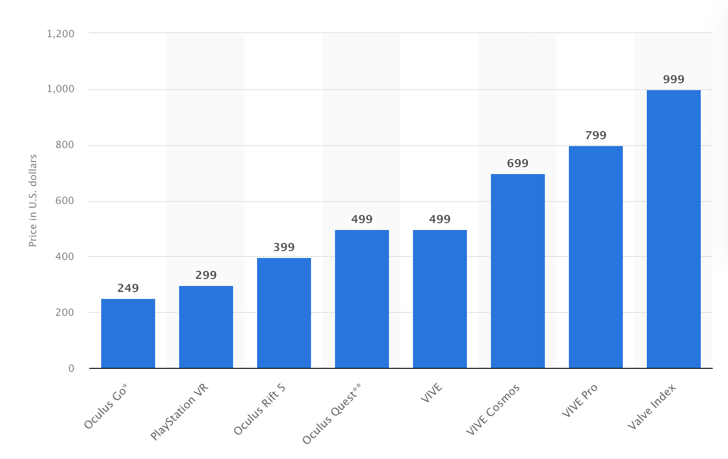
\includegraphics[scale=0.5]{pics/vr_headset_price_statistic}
    \caption{VR Headset Preise~\cite{ALSOP_2019}}
    \label{fig:vr_headset_prices}
\end{figure}

\subsubsection{Valve Index}

Die Valve Index ist eine VR-Brille welche von Valve entwickelt worden ist.
Diese befindet sich genauso wie die HTC Vive Pro~\ref{sec:htc-vive} im teureren Spektrum~\cite{ALSOP_2019} der VR-Brillen und ist dem Typ tethered Headset~\ref{sec:vr-headset-types} zuzuordnen.

\paragraph{Vorteile}

\begin{itemize}
    \item Hand Tracking.
    Die Controller tracken die Finger- und Handbewegungen.
    Diese Technologie kann von Spieleentwicklern verwendet werden~\cite{SadlyItsBradley_2019}
    \item lighthouse tracking (siehe HTC Vive)
\end{itemize}

\paragraph{Nachteile}

\begin{itemize}
    \item längerer Aufbau wie die Folgend beschriebene Oculus Quest 2
    \item hoher Preis~\ref{fig:vr_headset_prices}
    \item es wird ein Computer benötigt
\end{itemize}

\subsubsection{Oculus Quest 2}\label{sec:oculus-quest-2}

Die Oculus Quest 2 ist eine VR-Brille welche von Facebook/Meta im Jahre 2020 entwickelt worden is~\cite{ADI_ROBERTSON_2020}.
Diese Brille ist eine Mischung von einem tethered Headset und einem Standalone Headset~\ref{sec:vr-headset-types}.
Dies bedeutet, dass die Oculus Quest 2 ohne einen Computer benutzbar ist, aber auch mit einem USB-C Kabel zu einem Computer verbunden werden kann.
Ist das Headset mit dem Computer verbunden können PC exclusive Spiele mit der Oculus Quest 2 auch gespielt werden~\cite{ADI_ROBERTSON_2020}
Für den Aufbau werden nur das Headset und zwei Controller benötigt.

\paragraph{Vorteile}

\begin{itemize}
    \item Aufbauen erfordert keinen großen Aufwand.
    \item Die Brille befindet sich eher im unteren Preisspektrum der VR-Brillen~\ref{fig:vr_headset_prices}.
    \item es wird kein Computer benötigt
\end{itemize}

\paragraph{Nachteile}

\begin{itemize}
    \item Das Headset ist von natürlichem Licht abhängig~\cite{Dennis_Ziesecke_2019}
    \item Full Body Tracking kann etwas kompliziert und teuer werden~\cite{Martin_Rakver}
    \item weniger genaues Tracking~\cite{Macedo_2020}
\end{itemize}

\subsection{VR Controller}\label{sec:vr-controller}

\subsection{Tracker}\label{sec:tracker}

\subsubsection{Vive Tracker}\label{sec:vive-tracker}

\subsection{Lighthouse}\label{sec:lighthouse}

Die HTC Vive Brillen und die Valve Index benützen beide das Lighthouse-Tracking.
Diese Form des Trackings ist genauso wie bei der Oculus Quest und Oculus Quest 2 ein Inside-Out Tracking.
Im Gegensatz zu der Oculus Quest benützt das Lighthouse Tracking kein natürliches Licht, sondern für das Auge unsichtbares Licht, welches von den Lighthouses ausgestrahlt wird.


Dies hat den Vorteil, dass die Benutzung der Vr Brille nicht von dem natürlichen abhängig ist.
Statt Kameras besitzt ein zu trackendes Gerät Fotosensoren.
Im Falle der HTC Vive befinden sich diese Sensoren in den Einkerbungen der Brille.



\subsection{Wireless Adapter }

\section{Software}

\subsection{Game Engine}

Es gibt mehrere Games Engines mit welchen eine VR Applikation entwickelt werden kann.
In Abb.~\ref{fig:game_engine_marketshare} ist der Marktanteil verschiedener Engines abgebildet.
Diese Daten sind aber mit Vorsicht zu genießen, da das Skript welche diese Daten geliefert hat nach einigen Kriterien handelt,(siehe~\cite{REDDIT_2018}).
Dies bedeutet beispielsweise, dass nur Spiele mit einer Wikipedia Seite mit einberechnet werden.

\begin{figure}
    \centering
    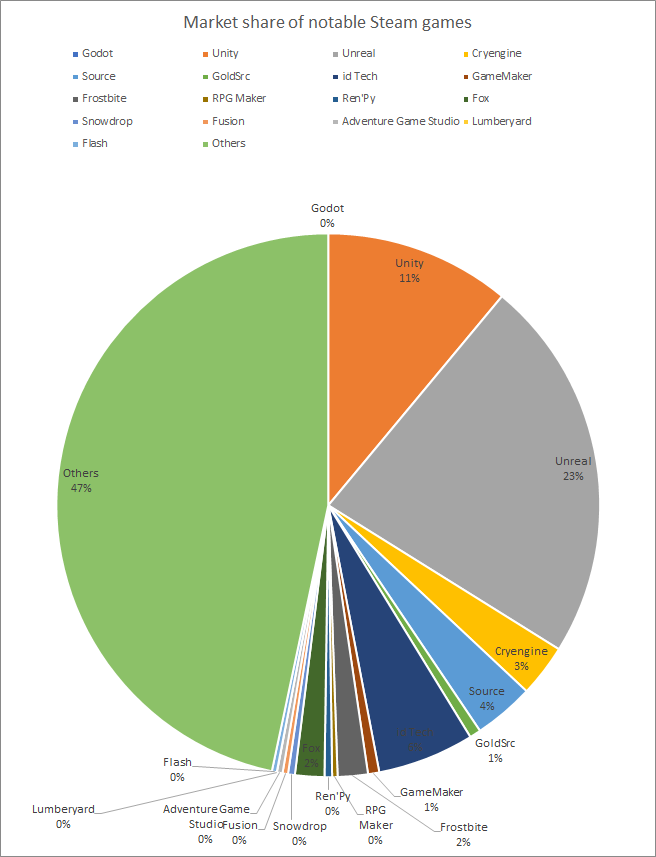
\includegraphics[scale=0.4]{pics/game_engine_marketshare}
    \caption{Game Engine Market-share~\cite{REDDIT_2018}}
    \label{fig:game_engine_marketshare}
\end{figure}

\begin{figure}
    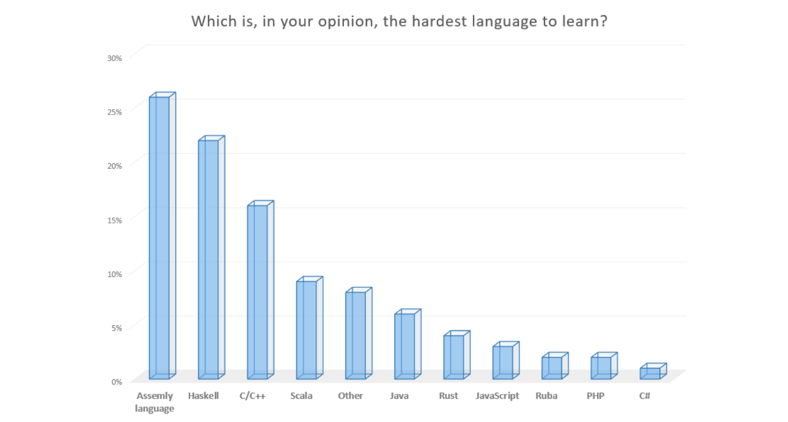
\includegraphics[scale=0.4]{pics/programming_languages_hardest}
    \caption{Schwerste Programmiersprachen~\cite{JAXCENTER_2018}}
    \label{fig:hardest_programming_languages}
\end{figure}

\subsubsection{Unity}

Unity ist eine Game Engine, welche von Unity Technologies initial exklusiv für Apple Mac OS X entwickelt wurde.
Die Engine wurde portiert und kann heute auch auf Windows und auf der Linux Plattform benützt werden.
Sie ist für alle im prinzip gratis bis zu einem bestimmten Umsatz.
Auch wenn sie eine Einsteiger Engine genannt wird, ist sie trotzdem im professionellen Bereich in benutzung und viele bekannte Spiele, wie Pokemon GO, Among us und Hearthstone wurden in der Unity Engine entwickelt~\cite{Haas2014AHO,UNITY_DOWNLOAD,UNITY_PRICING,WIKIPEDIA_UNITY_GAME_LIST_2014}.

\paragraph{Vorteile}

\begin{itemize}
    \item Gratis benutzung bis zu einem bestimmten Umsatz eines Produktes
    \item Programmierbar in C\#, einer einfach zu erlernenden Sprachen siehe Abb.~\ref{fig:hardest_programming_languages}
    \item Es kann für alle möglichen Plattformen ein Programm geschrieben werden~\cite{UNITY_PLATTFORMS}
    \begin{itemize}
        \item IOS
        \item Android
        \item Windows
        \item Linux
        \item WebGL
    \end{itemize}
\end{itemize}

\paragraph{Nachteile}

\begin{itemize}
    \item im Vergleich zu Unreal weniger Market-share~\ref{fig:game_engine_marketshare}
    \item geschlossener Source Code
    \item schnellerer Kostenanfall wie bei Unreal
\end{itemize}

\subsubsection{Unreal Engine}
\label{sec:unreal_engine}

Unreal Engine wird von Epic Games entwickelt~\cite{UNEAL_ENGINE_OWNER_2022}.
Diese Engine ist eine weit verbreitete Game Engine.
Dies kann man Abbildung~\ref{fig:game_engine_marketshare} entnehmen.
Viele Spiele wie Fortnite, Ark Survival Evolved, Borderlands 3 und Jedi Fallen Order sind mit dieser Engine entwickelt worden~\cite{WIKIPEDIA_UNREAL_GAME_LIST}.

\begin{figure}
    \centering
    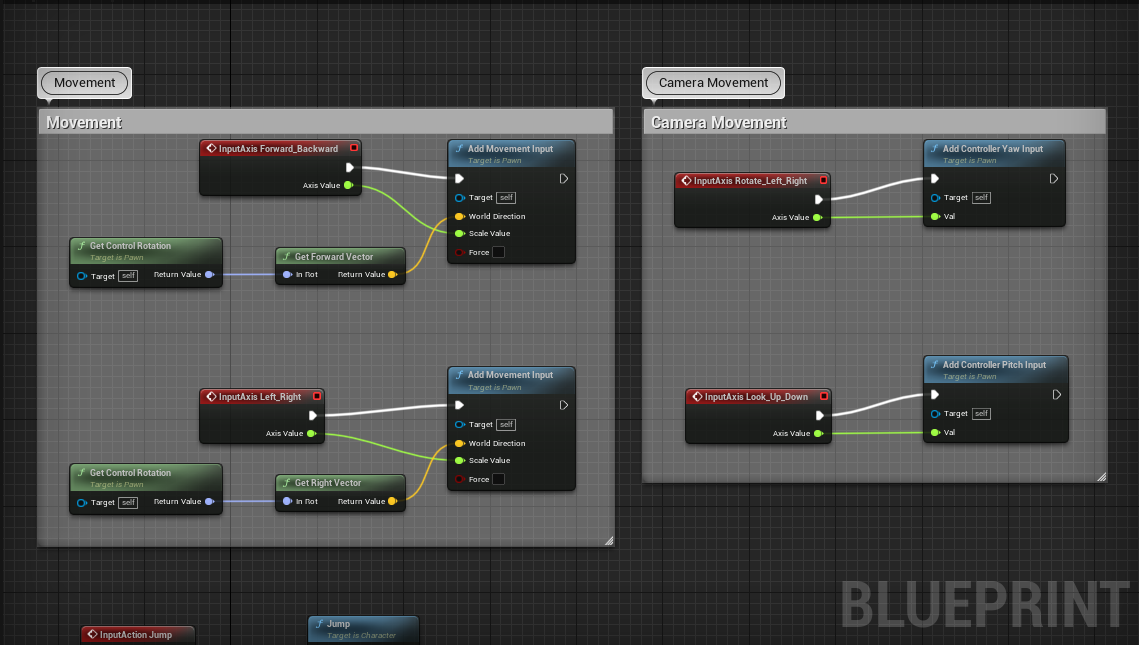
\includegraphics[scale=0.3]{pics/visual_scripting_unreal_engine}
    \caption{Visual Scripting in Unreal Engine 5}
    \label{fig:visual_scripting_unreal_engine}
\end{figure}

\paragraph{Vorteile}

\begin{itemize}
    \item höchster Market-share nach Abb.~\ref{fig:game_engine_marketshare}
    \item 'easy to learn' visual scripting~\ref{fig:visual_scripting_unreal_engine} %TODO: Statistic for visual scripting vs Code
    \item Lizenzkosten von 5\% folgen erst bei einem Einkommen durch ein Produkt von 1.000.000\$~\cite{UNREAL_ENGINE_PRICING_2022}
\end{itemize}

\paragraph{Nachteile}

\begin{itemize}
    \item 5\% Lizenzkosten, wenn das Einkommen eines Produktes über 1.000.000\$ ist~\cite{UNREAL_ENGINE_PRICING_2022}
    \item für erweiterte Funktionalität wird C++ benötigt, welches nach Umfrage in Abbildung~\ref{fig:hardest_programming_languages} die drittschwierigste Sprache zu erlernen ist
\end{itemize}

\subsubsection{Source Engine und Source 2 Engine}

Es gibt mittlerweile 2 Iterationen dieser Engine.
Zum einen die originale Source Engine und die Source Engine 2.
Die Markteinführung der ursprünglichen Source Engine war im Juni 2004~\cite{Bryan_Wirtz_SOURCE_ENGINE_2022}.
Daraufhin ist die Source 2 Engine im August 2014 erschienen~\cite{VALVE_DEVELOPER_COMMUNITY_SOURCE2}.
Beide Engines sind von Valve entwickelt worden~\cite{VALVE_DEVELOPER_COMMUNITY_SOURCE, VALVE_DEVELOPER_COMMUNITY_SOURCE2}.
Verantwortlich ist die Source 2 Engine für Spiele wie Dota 2 und Half Life Alyx~\cite{WIKIPEDIA_SOURCE2_ENGINE_GAME_LIST}.
Andere Spiele wie Half Life 2, Counterstrike Source, Portal, Portal 2 und Counterstrike Global Offensive sind mit der originalen Source Engine entwickelt worden~\cite{WIKIPEDIA_SOURCE_ENGINE_GAME_LIST}.
Auch als VR Entwicklungsumgebung eignet sich die Source 2 Engine, da sie für Half Life: Alyx, eines der erfolgreichsten VR Spiele benutzt worden ist~\cite{WIKIPEDIA_SOURCE2_ENGINE_GAME_LIST, Aden_Carter_2020}.
Die folgenden Vorteile und Nachteile beziehen sich auf die Source 2 Engine.

\paragraph{Vorteile}

\begin{itemize}
    \item Source Engine ist gratis zu nutzen und zu publizieren *(siehe Nachteile)
\end{itemize}


\paragraph{Nachteile}\label{pgr:cons}

\begin{itemize}
    \item kein hoher Market-share (siehe Abbildung~\ref{fig:game_engine_marketshare})
    \item spiele, welche mit der Engine entwickelt worden sind, dürfen nur auf Steam publiziert werden~\cite{Brenna_Hillier_2015}
\end{itemize}



\subsection{VR Plugin}

\subsection{Steam}

\subsection{Vive Wireless}

\subsection{Final IK Plugin}

\subsection{IDE}

\subsection{Modellierung}
